\noindent
The healthcare systems of the future will be highly decentralised, integrating home-, work- and environment-based monitoring systems with existing hospital diagnostic systems. The benefits of integrating such a variety of systems and information on patients include a reduction of costs and travel-associated risks while allowing patients to get faster diagnostics and better medical treatments that more accurately suit their needs. %(cf. Figure~\ref{fig:dataExch}).
As a consequence, medical data will need to be collected from a variety of sources and exchanged in a variety of ways, including over public networks that cannot be implicitly trusted. At the same time, however, we have stricter regulations on ownership and handling of personal data. Transnational standards for data protection, such as the EU General Data Protection Regulation\footnote{Information on GDPR can be found at https://gdpr-info.eu/}, will need to be combined with local regulations, giving very strict rules about who is allowed to access (parts of) patient data. Complying with data protection regulations whilst facilitating data exchange and analytics in a decentralised way is a key challenge for future healthcare systems.

%\begin{figure}[t!]
%    \centering
%    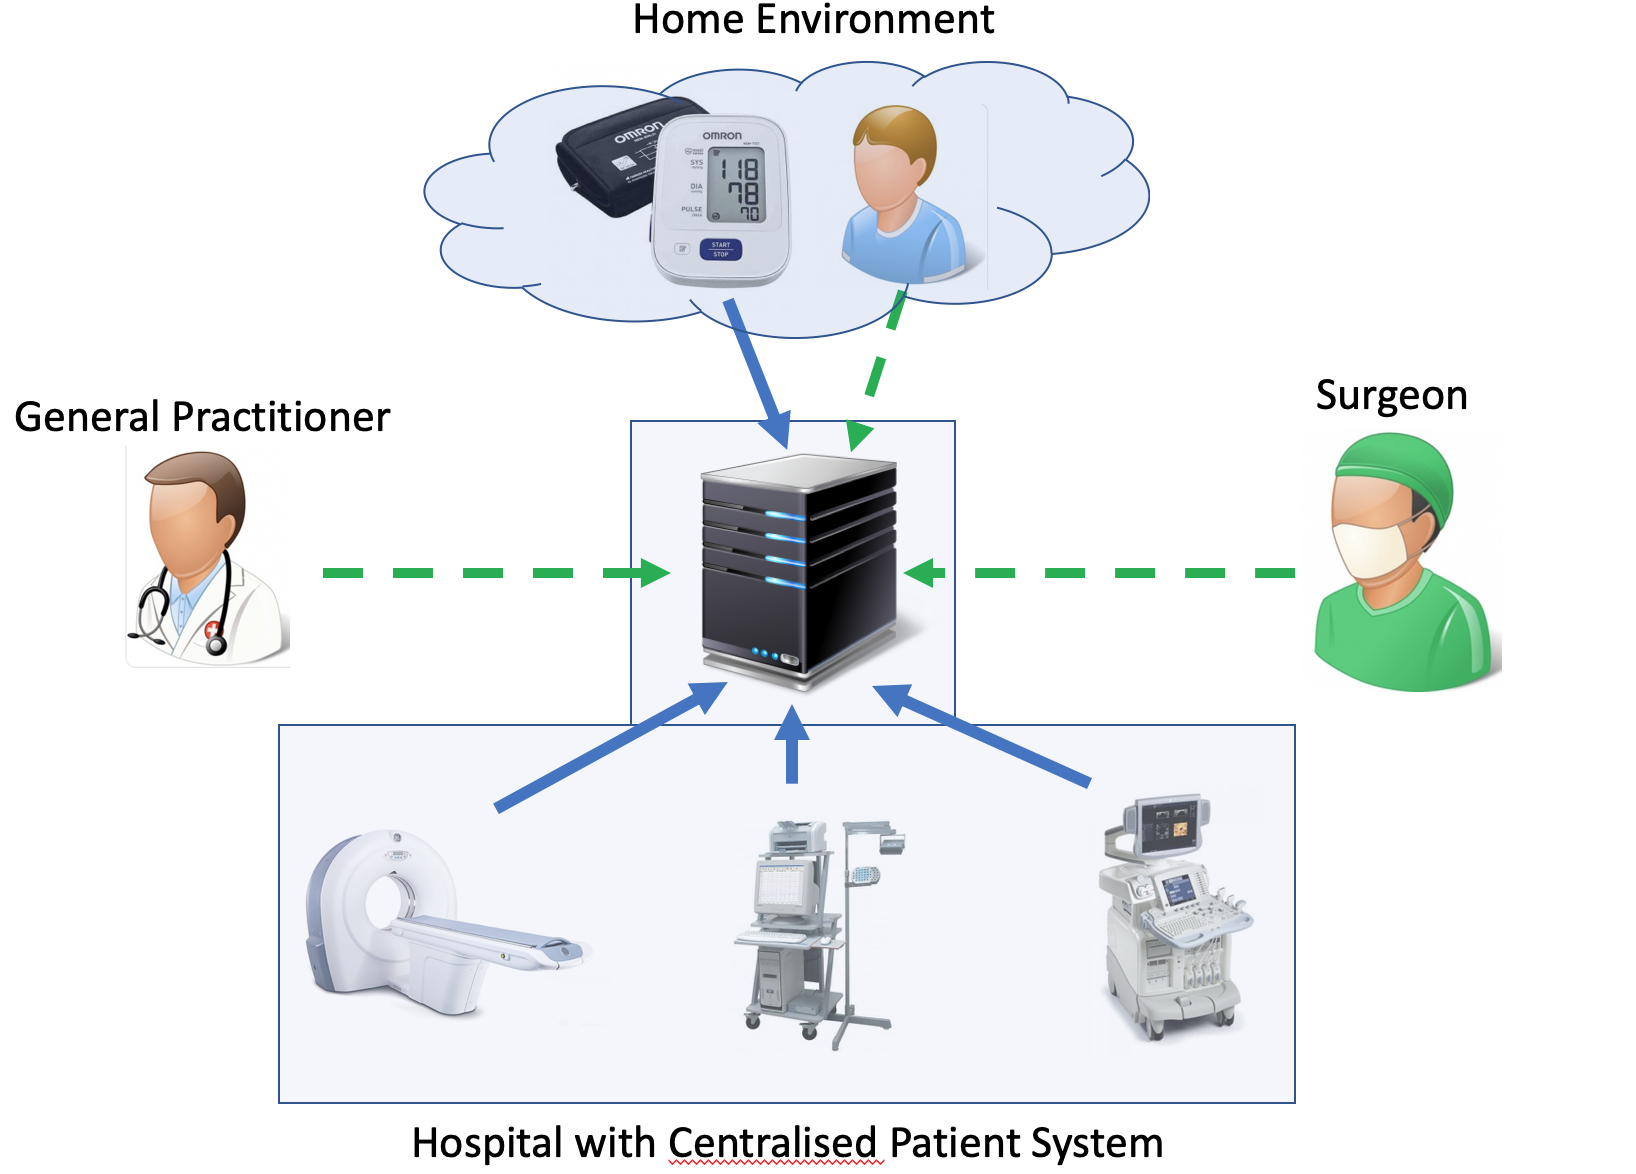
\includegraphics[width=70mm]{images/DataExchange.png}
%    \caption{Data Exchange in Modern Healthcare Systems}
%    \label{fig:dataExch}
%\end{figure}

In this paper, we describe a methodology and complete tool-chain that will be developed over the course of the ongoing EU H2020 project \emph{SERUMS}\footnote{Securing Medical Data in Smart Patient-Centric Healthcare Systems (SERUMS): https://serums-h2020.weebly.com} to address  safe, secure and privacy-preserving storage, access, communication and analysis of the medical data in future-generation smart health centres. Our main goal is to put patients at the centre of the future healthcare provision in Europe, enhancing their personal care and maximising the quality of treatment that they will receive, whilst ensuring trust in the security and privacy of their confidential medical data. 
%To this end, we aim to develop a complete tool-chain that will ensure the security and privacy of data over its lifetime, from collection  onward through envisaged and future permitted analytics.

To reduce the scope of the paper, we restrict our attention to a subset of the \emph{SERUMS} technologies. We propose a \emph{universal format} for patient records, to allow a uniform representation of patient data across different use cases and describe its implementation.
%using the \emph{data vault} concept from data science. 
We describe \emph{FlexiPass}, an authentication mechanisms to access these records, together with the application of \emph{blockchain technology} to control permissions, ensuring that only allowed staff have access to required parts of patient records, 
%and processed within a \emph{data lake}, 
and to save the access history of all records. We describe a novel, \emph{privacy-preserving} data analytics mechanism which ensures that the analytics model itself does not accidentally leak sensitive information. Finally, we present a \emph{data fabrication} approach that allows the generation
of synthetic but realistic data, given 
a strict format of patient records and dependency rules between its elements. In the context of the SERUMS project, we only use generated synthetic data for the development and verification of our technologies, but we will furthermore prove formally the \emph{closeness} of the synthetic and real data.
% HERE is where we should mention verification technologies
For illustration, we present one of SERUMS real-world use cases on predicting toxicity levels of cancer treatments. 
%from the Edinburgh Cancer Centre (ECC), NHS Lothian. 

%This paper is structured as follows...

%This paper makes the following concrete research contributions: 
%\begin{itemize}
%    \item We propose a \emph{SERUMS} methodology, with the associated %interoperable tool-chain for management and analytics of confidential medical %data in modern distributed healthcare systems;
%    \item We describe initial implementations of the tools from the %\emph{SERUMS} tool-chain;
%    \item We evaluate the \emph{SERUMS} tool-chain on \emph{Edinburgh Cancer %Gateway}, a real-world use case for predicting toxicity levels of cancer %treatments. 
%\end{itemize}


\section{Background}

\noindent
The emergence of Internet-of-Things (IoT) technology is having a profound effect on the development of modern healthcare systems. Traditionally healthcare systems were highly centralised with data relevant to a  patient,  as well as the devices used to obtain this data (e.g., blood pressure monitors, CT scanners), residing in a central location, for example within a hospital. 
From a security and privacy point of view, collecting, storing and processing such data was relatively simple, since the data only needed to be communicated over trusted networks. 
However, as personal medical devices become cheaper and more prevalent, 
%it became clear that integrating home-based healthcare, with all of its advantages such as wearable devices with home monitoring sensors, into the holistic diagnostics and treatment plan for patients can significantly reduce cost and travel-associated risks while increasing the quality of healthcare provision. This, however, involves 
and there is an increased realisation of the benefits of integrating 
a variety of health data sources for improved healthcare provision, new significant challenges emerge with  
sharing private and confidential data across public networks.
%posing significantly more risk than when the data is only exchanged within a single trusted organisation. This scenario also presents a number of additional issues that need to be dealt with.
In particular, we need to be able to ensure:
\begin{itemize}
 %   \item \emph{Ensuring Trust}. The patients must have a high degree of trust both that the smart healthcare system operates as intended, and that their privacy is fully protected.
  %  \item \emph{Security, Privacy and Anonymity}. The smart healthcare system must work efficiently as a whole in order to maximise the quality of patient care, yet must simultaneously provide high levels of security and support high expectations of privacy and anonymity.
   % \item \emph{Control of the data}. The patients must have full control of their data, as required by the GDPR and other legislation, yet the data must be provided in a timely fashion to medical practitioners and specialists.
    %\item \emph{Compliance to regulations.} In order to support emergency medicine or other forms of trans-border medical treatment, the smart healthcare system must comply with with multiple, possibly conflicting, legislative frameworks.
    \item \emph{Trust}: Patients must be able to trust that systems operate as intended and that their data is fully protected.
    \item \emph{Security, Privacy and Anonymity}: Systems must operate efficiently and guarantee  the best possible quality of healthcare, whilst simultaneously providing high levels of security and expectations on data privacy and anonymity.
    \item \emph{Data Control}: Patients must have full control of their data according to expectation and law, whilst allowing medical staff data access as required.
    \item \emph{Regulation Compliance}: The smart healthcare system must comply with regulations at various levels, including 
    %those that support the points above such as 
    GDPR, local legislation and policy that may at times conflict with the above goals or other legislation.
\end{itemize}
SERUMS tackles the above problems by (1) addressing security and protection of shared medical data across untrusted networks;
(2) integrating personal medical data, coming from various sources, into coherent and structured smart patient records;
(3) enabling data analytics techniques over distributed data; and
%    \item 
(4) developing authentication and trust mechanisms that will ensure that only properly authorised staff have access to (parts of) personal and medical data. At the same time, we consider
world-leading levels of compliance to existing and emerging legal and ethical standards.
%\subsection{The SERUMS Project}

%\noindent
%\emph{SERUMS: Securing Medical Data in Smart Patient-Centric Healthcare Systems} is a recently-started \texteuro4.47M EU H2020 project that aims to produce tools and techniques for safe and secure collection, storage, communication and processing of health data. SERUMS includes three universities (University of St Andrews from Scotland, University of Cyprus and Universite Catholique de Louvain from Belgium), four industrial technology providers (IBM Science and Technology from Israel, Sopra Steria from the UK, Software Competence Center Hagenberg from Austria and Accenture BV from Netherlands) and two end-user healthcare Centres (Zuyderland Medisch Centrum from Netherlands and Fundacio Clinic per a la Recerce Biomedica from Spain). The goal of the project is to provide technologies for
%\begin{itemize}
%    \item Security and protection of the shared medical data across untrusted networks;
%    \item Integrating personal medical data, coming from various sources, into coherent and structured smart patient records;
%    \item Data analytics techniques that will be able to deal with distributed data that cannot be moved to a central location;
%    \item Authentication and trust mechanisms that will ensure that only properly authorised agents have access to the required part of personal and medical data;
%    \item World-leading levels of compliance to the existing and emerging legal and ethical standards.
%\end{itemize}

\section{SERUMS Tool-Chain} % For Smart Health Centre Systems}

% TGW: I made this figure larger as the text was too small to read otherwise. We can shrink and also wrapfig if we need space.
\begin{figure*}[ht!]
    \centering
    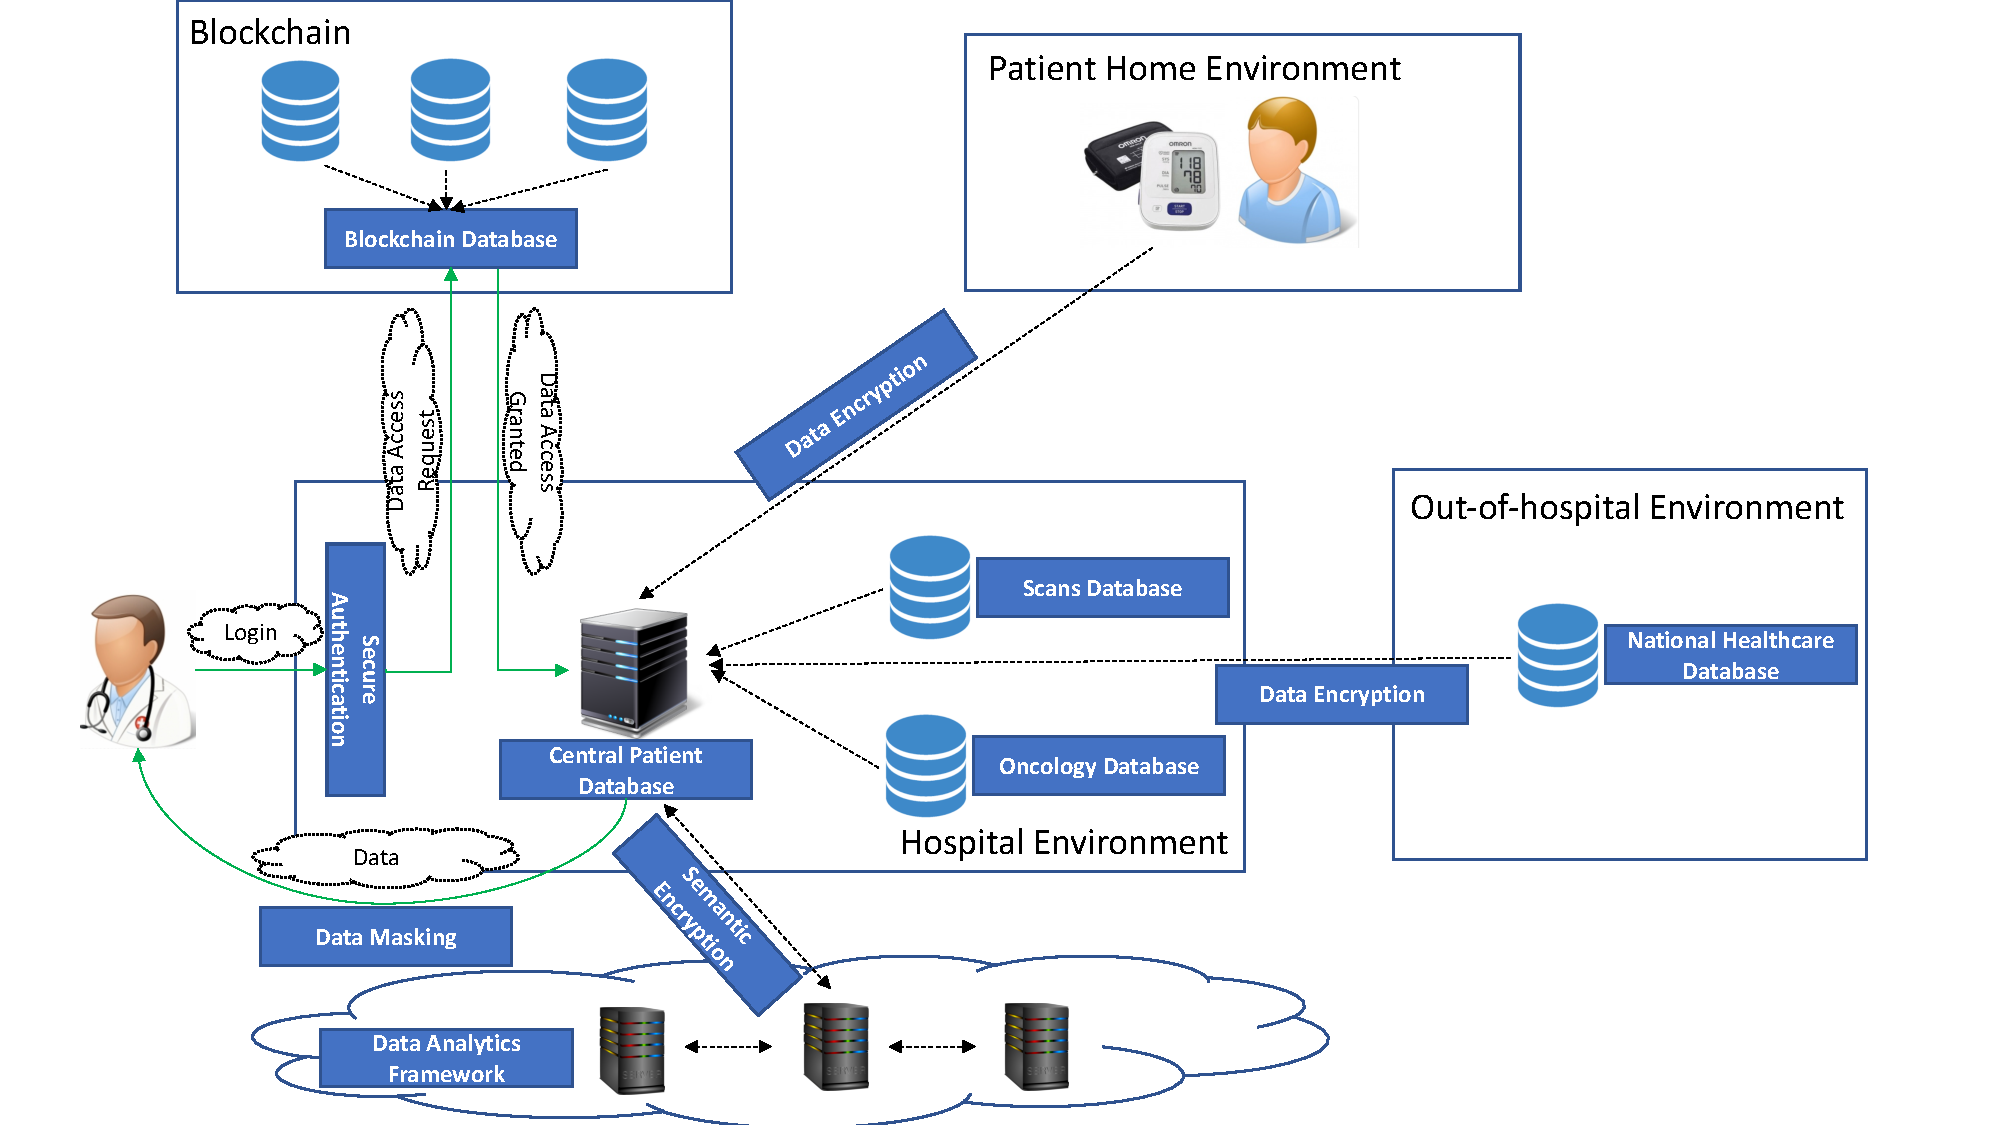
\includegraphics[width=140mm]{images/SerumsOverview.pdf}
    \caption{The overview of \emph{SERUMS} tool-chain}
    \label{fig:serumsTools}
\end{figure*}

\noindent Figure~\ref{fig:serumsTools} gives an overview of the \emph{SERUMS} tool chain and the overall process of accessing data across a distributed healthcare system. %and using the smart health centres that will be based on it. 
The core of it is a centralised data lake that holds the \emph{smart patient records} (see Section~\ref{sec:smartPatient}). Note that, while the patient records are centralised, the data in them may refer to databases distributed inside and outside of the hospital environment. These records contain all information about the patients, from static information such as date of birth, gender and contact information, to vital information such as weight, body mass index, allergies, to dynamic information about treatments and examinations. Some of the data for the records will be collected from within the healthcare system over trusted networks, while other may be collected from personal health monitoring devices, etc. Data sent over untrusted networks must be secured using \emph{data encryption} mechanisms.

%{\color{red}[TGW: above we talk about `static information'' but use examples that can change, e.g. gender and contact information, whereas weight and BMI may be more dynamic, it is still not clear what distinguishes static from dynamic here.] \color{red}[VJ: Static information is unlikely to change or it changes very rarely, while the dynamic information is changed/updated on every visit (e.g.list of received treatments). But we mention these two just to illustrate a variety of information that will be held in the records. We don't really make any difference with respect to the kind of data used in any of our technologies.]}

When staff needs to access patient data, they first log in to the central healthcare system using \emph{secure authentication} mechanisms. In the SERUMS project, our aim is to develop personalised and adaptive multi-factor user authentication schemes (see Section~\ref{sec:authentication}). Once the user logs in, their access rights are checked using the \emph{blockchain backend} which is linked to a distributed \emph{blockchain database}. Different classes of users (e.g.~patients, GPs, specialists, insurers) will have different levels of permissions, according to GDPR and other legal and ethical regulations. For example, the patient has full access to their record, while a specialist can only access parts of the record that are relevant to them. The blockchain ensures that only authorised agents can access the data, and depending on permissions, possibly only be part of the data. The blockchain contains all access rules and transitions, and keeps a record the data access history. Note, however, that no actual data is stored in the blockchain.

Once the user is authenticated and the access rights are checked, the requested data from the smart patient records data lake is sent back to the user. If the user does not have full access rights to the record, the data transfer may involve masking parts of the data, i.e., hiding parts of the record that the user has no access right to see. The access transaction itself is stored in the blockchain database.

Finally, different kinds of analysis will need to performed on patient data. In the \emph{SERUMS} project, we focus on deep learning analytics to drive diagnostics and prediction of treatment outcomes (see the use case in Section~\ref{sec:useCase}). Since the data referred to from the smart patient records is distributed, and we assume that some of this data cannot leave the place where it is stored, the analytics will also need to be performed in a distributed way. We need to make sure that no unsafe information is revealed by the learning models, as well as to ensure security of the data communicated between the central patient record database and the analytics model (which may reside in the cloud). In this context, our aim is to develop  \emph{privacy-preserving distributed deep-learning analytics models} for data analysis (see Section~\ref{sec:dataanalysis}).

%{\color{purple}[NEW]To ensure adequate privacy, correctness, and compliance with legislation the key SERUMS technologies will be validated and verified during design and development. This involves the verification of mechanisms to ensure the behaviours above, and of the SERUMS implementation.}

For the purposes of developing, verifying, and testing the complete \emph{SERUMS} infrastructure, the SERUMS project will use \emph{synthetic} instead of real patient data, to avoid any privacy and security concerns. \emph{Data fabrication} (See Section~\ref{sec:datafabrication}) technology allows us to rapidly generate large volumes of data that is the same in terms of structure as real data, but which was synthetically generated. The strict format of the smart patient records, the formally defined rules on possible values for each field, the relationships between different fields and the well-formulated data interaction rules, makes it possible to automate this process. 




%Next we go into details on the individual methodologies within the SERUMS tool-chain.

%\section{SERUMS Technologies}

%\subsection{Smart Patient Records}
%\label{sec:smartrecords}


%\subsection{Data Fabrication}
%\label{sec:datafabrication}

%\subsection{Data Masking}
%\label{sec:datamasking}

%\subsection{Distributed Privacy-Preserving Data Analytics}
%\label{sec:dataanalysis}

%\subsection{Authentication and Authorisation}
%\label{sec:authentication}

%\subsection{Blockchain Smart Contracts}
%\label{sec:blockchain}



%\section{Evaluation}

%\subsection{Use Case Description}
%\label{usecase}





%\subsection*{Notes}

%Here are the items from the call for Healthcare Data and some comments/notes:
%\begin{enumerate}
%\item 
%\emph{Health data collection and analysis:}
%We have a lot of basis on this, we are clearly in both collection analytics.

%\item 
%\emph{Problems in health data processing:}
%We have some data processing aspects, so this is also strong for us.

%\item 
%\emph{Protection and security of personal health data:}
%We have this conceptually, and also concrete connections to GDPR.

%\item 
%\emph{Electronic health records and standards:}
%Exactly what we're doing for the first parts, standards not so clear?

%AV - suggest?

%COMMISSION RECOMMENDATION (EU) 2019/243 
%European Electronic Health Record exchange format 

%https://www.hl7.org/
%http://www.hl7.org/fhir/

%\end{enumerate}



